\documentclass[conference]{IEEEtran}

\usepackage{booktabs}
\usepackage{graphicx}
\usepackage{tabularx}
\usepackage{url}
\usepackage[hidelinks]{hyperref}
\newcolumntype{Y}{>{\raggedright\arraybackslash}X}
\Urlmuskip=0mu plus 1mu
\emergencystretch=2em

\title{Evidence Visibility Shapes Risk Behavior in a Controlled LLM Patch-Verifier Study}
\author{\IEEEauthorblockN{Anonymous Authors}\IEEEauthorblockA{Anonymous Institution}}

\begin{document}
\maketitle




\begin{abstract}

Patch-verification decisions made by large language models (LLMs) are meaningful only relative to the evidence visible at review time. Existing evaluations often report whether an LLM accepts or rejects a patch without making this evidence boundary explicit, which makes it difficult to separate model capability from visible-test evidence, tool-summary anchoring, or prompt-induced caution. This paper introduces the Evidence-Visibility Protocol (EVP-8), a hidden-evaluator protocol for candidate patch verification. EVP-8 reviews 98 candidate patches across seven cumulative evidence levels while withholding evaluator-only correctness labels until post-decision analysis. In three repaired v0.3 runs, Qwen reached 95.24\% E6 correct recall with 83.33\% accepted precision, DeepSeek reached 80.95\% E6 correct recall with 80.95\% accepted precision, and Gemini reached 95.24\% E6 correct recall with 80.00\% accepted precision. The three models still accepted 4-5 of 77 non-correct candidates at E6. E6 ablations, current-98 coverage-contestation, and a 31-case hard-negative stress matrix show that prompt framing can strongly shift risk policy: in the stress matrix, coverage-contestation reduced repeated false accepts from 62/93 to 12/93, entirely through escalation rather than strict rejection. These results support a bounded software-engineering claim: in this controlled LLM patch-verifier study, evidence visibility should be treated as an experimental variable for risk control, not as proof of general autonomous correctness verification.

\end{abstract}
\section{Introduction}

Automated patch generation and LLM-assisted review are increasingly positioned near software merge decisions. This creates a practical software-quality question: when a candidate patch appears plausible, which visible evidence is sufficient for a verifier to accept it rather than reject it or escalate it for human review? Prior automated program repair work has shown that plausible or test-passing patches can still be incorrect \cite{qi_issta_2015_patch_plausibility,legoues_icse_2012_genprog}, so a merge decision cannot be reduced to surface plausibility alone.

The difficulty is not only whether an LLM can read code. It is that a verifier's decision may change when issue context, patch structure, static status, visible tests, regression checks, diagnostics, or tool summaries become visible. If these evidence fields are not controlled, an evaluation may conflate model judgment with evidence presentation. In particular, authoritative-looking tool summaries can encourage acceptance even when the underlying semantic correctness remains unknown.

This paper studies candidate patch verification as an evidence-conditioned merge-gate task. A verifier receives a candidate patch and a predefined model-visible evidence packet, then emits one of three decisions: accept, reject, or escalate. Correctness labels and hidden evaluator outcomes are joined only after the decision. This design follows the intuition behind reject-option and selective-classification settings \cite{chow_tit_1970_reject_option,geifman_el_yaniv_2017_selective_classification}, but applies it to software patch verification. The current empirical scope is intentionally controlled: the paper-facing main result is a three-model repaired v0.3 analysis for Qwen, DeepSeek, and Gemini, supported by E6 ablations and tool-contestation evidence, rather than a broad claim about all LLM verifiers.

The paper makes three contributions:

\begin{itemize}
\item It defines EVP-8, a hidden-evaluator evidence-visibility protocol for measuring accept, reject, and escalation behavior in candidate patch verification.
\item It reports repaired Qwen, DeepSeek, and Gemini v0.3 label-conditioned results showing that visible executable and tool evidence can unlock correct-patch acceptance while introducing bounded false-accept risk.
\item It analyzes E6 rule-only, no-verdict, tool-contestation, coverage-contestation, and hard-negative stress-test conditions to separate deterministic tool evidence, verdict-like anchoring, safe handling, strict correction, and prompt-induced conservatism.
\end{itemize}

The claim is deliberately bounded. The results do not establish reliable autonomous patch correctness verification, nor do they show that LLM decisions consistently outperform deterministic baselines. They show that evidence visibility is a measurable experimental variable that should be controlled and reported in LLM patch-verifier studies.

\section{Background and Motivation}

Automated program repair research has long distinguished plausible patches from correct patches. Generate-and-validate systems and controlled benchmarks have shown that passing available tests may be insufficient for semantic correctness \cite{qi_issta_2015_patch_plausibility,just_issta_2014_defects4j}. EVP-8 studies the downstream verifier setting: after a candidate patch exists, the question is not how it was generated, but whether a merge-gate decision is justified by the evidence visible to the verifier.

Software testing research also motivates the hidden-evaluator design. The oracle problem means that deciding correctness is itself a validity boundary \cite{barr_tse_2015_oracle_problem}. EVP-8 therefore keeps evaluator-only labels separate from model-visible evidence and joins them only after decisions have been produced.

LLM-based repair and code-editing studies show that LLMs can produce or inspect patches \cite{xia_zhang_icse_2023_llm_apr,tufano_icse_2019_bugfix_nmt}. However, verifier behavior is not identical to generation performance. A patch reviewer must decide whether visible evidence is enough to accept, reject, or escalate. This makes the task closer to code review and risk triage than to benchmark success alone \cite{bacchelli_bird_icse_2013_code_review}.

Finally, LLM-as-judge and automation-reliance work warn that model judgments and automation outputs require controlled protocols and explicit boundaries \cite{zheng_neurips_2023_llm_judge,parasuraman_riley_1997_automation}. The protocol in this paper responds to that concern by making evidence visibility an explicit variable rather than an implicit property of the prompt.

\section{Evidence-Visibility Protocol}

EVP-8 evaluates a candidate patch under a fixed evidence packet. The model-visible packet contains only the evidence level assigned to that condition. The evaluator-only layer contains hidden correctness labels and oracle outcomes used only after the verifier emits its decision.

\begin{figure}[t]
\centering
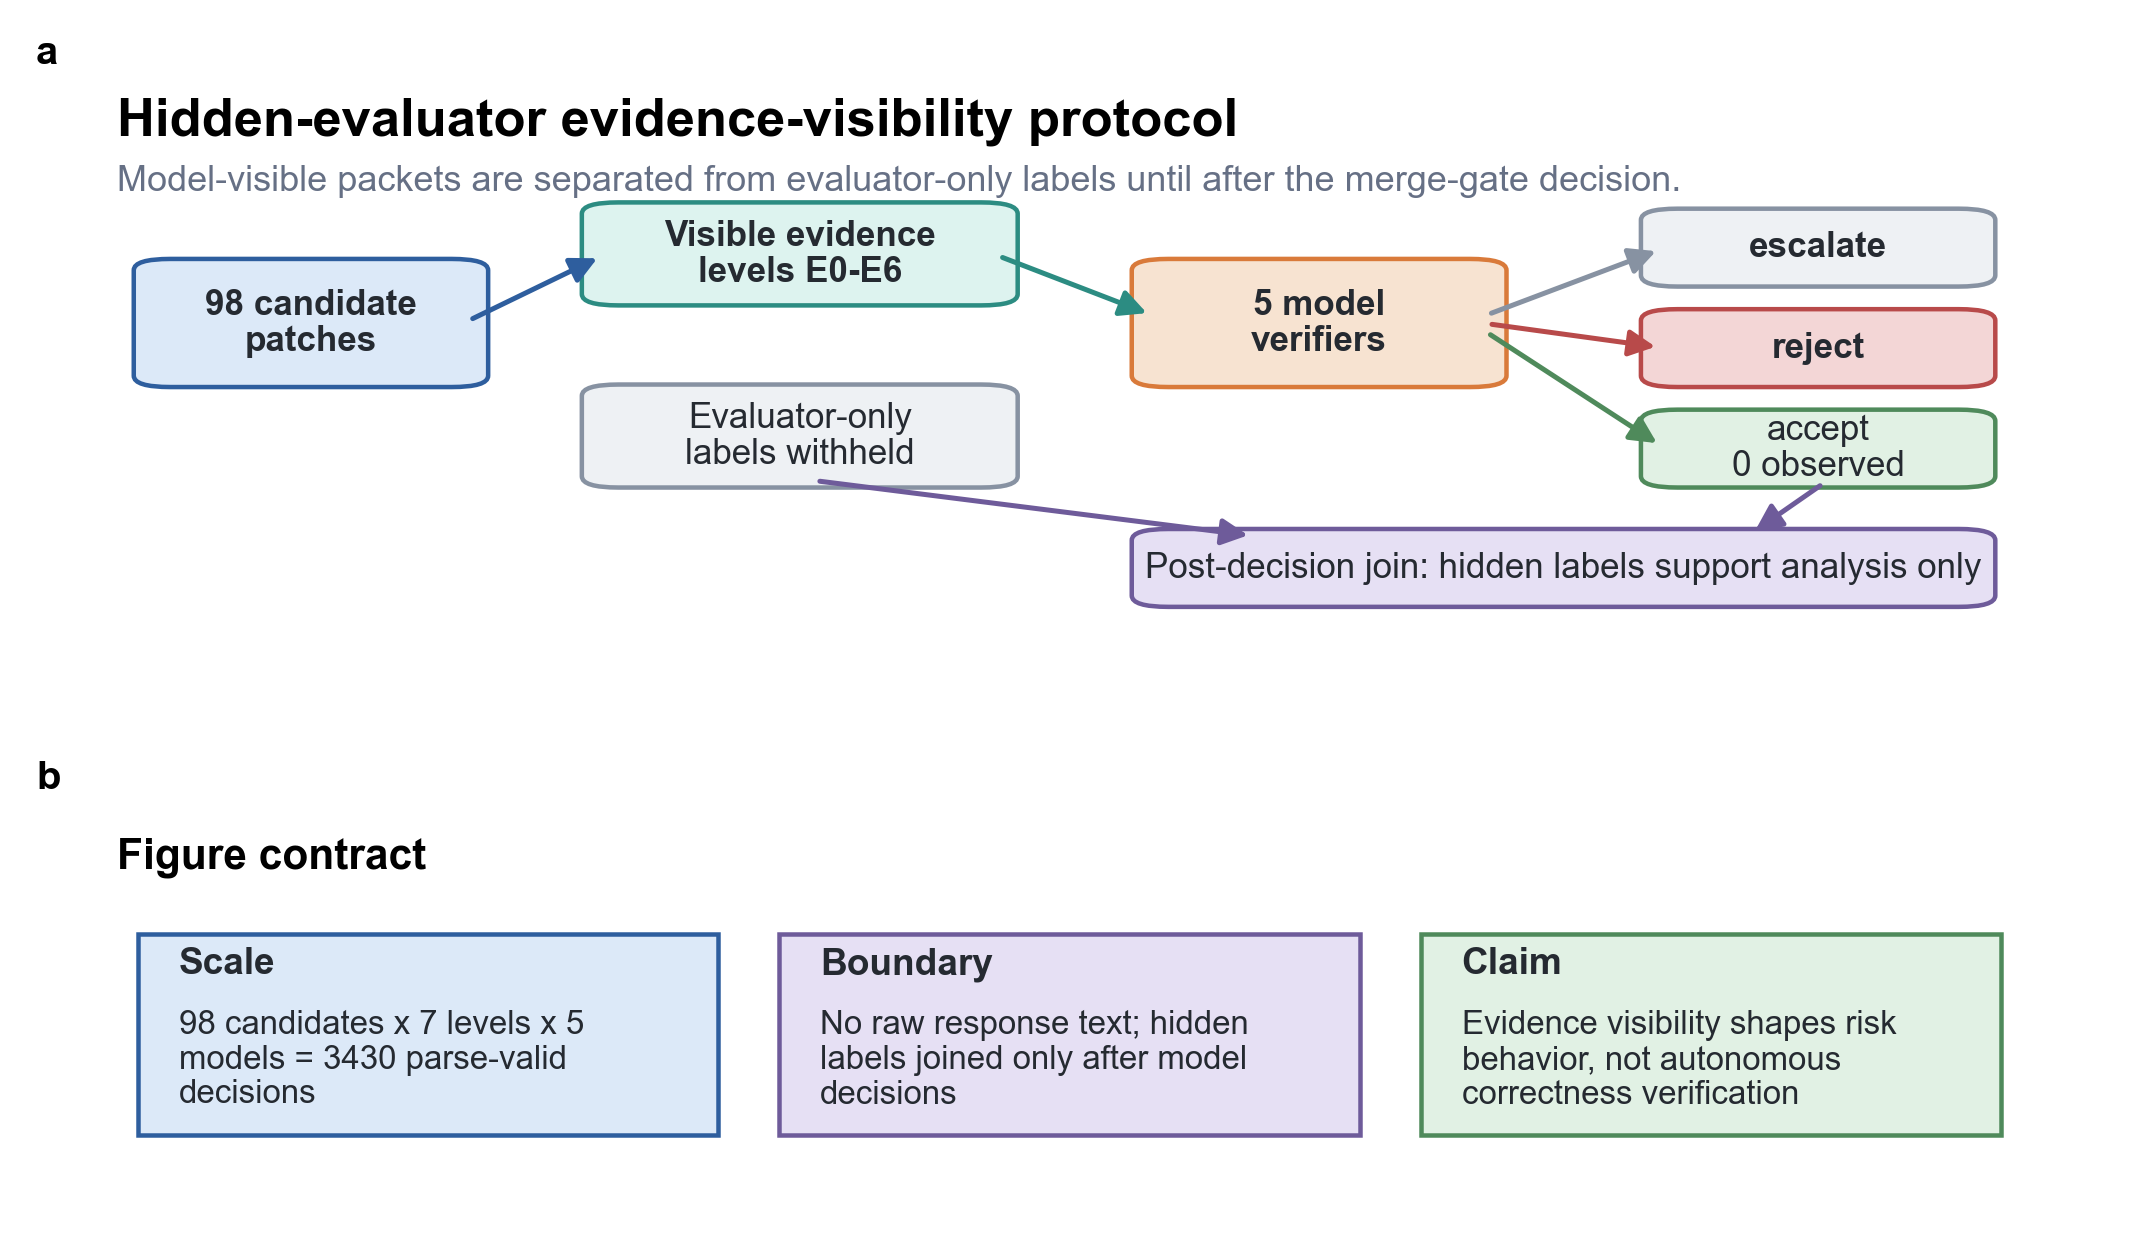
\includegraphics[width=\columnwidth]{../figures/ccfc/ccfc_fig1_protocol.png}
\caption{Hidden-evaluator evidence-visibility protocol.}
\label{fig:apsec-1}
\end{figure}

The reviewed unit is a candidate patch. The decision space is accept, reject, or escalate. Escalation is treated as a human-review routing decision, not as semantic rejection. This distinction is important because safe handling of a risky patch can occur through escalation even when strict correction does not occur.

EVP-8 uses seven cumulative evidence levels:

\begin{table*}[t]
\centering
\scriptsize
\setlength{\tabcolsep}{2pt}
\caption{Cumulative EVP-8 evidence levels.}
\label{tab:apsec-1}
\begin{tabularx}{\textwidth}{YYY}
\toprule
level & visible evidence & meaning \\
\midrule
E0 & Issue summary and candidate patch diff & minimal review context \\
E1 & Structured \path{changed-file/function} map & patch surface information \\
E2 & Patch application and static-check status & basic feasibility evidence \\
E3 & Visible fail-to-pass test results & \path{issue-relevant} executable evidence \\
E4 & Visible pass-to-pass regression results & \path{regression-safety} evidence \\
E5 & Additional diagnostics & broader tool evidence \\
E6 & Deterministic merge-gate summary & summarized tool verdict \\
\bottomrule
\end{tabularx}
\end{table*}

The current packet set contains 98 candidate patches from 6 projects and 21 BugsInPy tasks. It contains 21 correct patches and 77 non-correct patches under hidden F2P/P2P-broad evaluator labels. The candidate mix is intentionally skewed toward negative and partial cases because the merge-gate risk is false acceptance rather than classification accuracy on a balanced benchmark.

\begin{table*}[t]
\centering
\scriptsize
\setlength{\tabcolsep}{2pt}
\caption{EVP-8 candidate composition.}
\label{tab:apsec-2}
\begin{tabularx}{\textwidth}{YYYYYY}
\toprule
candidate type & count & evaluator label & label count & label source & purpose \\
\midrule
Correct reference & 21 & Correct under F2P and P2P-broad & 21 & hidden F2P and P2P-broad evaluator labels & measure correct-patch recall \\
Buggy no-op & 21 & Issue not fixed & part of 76 \path{issue-not-fixed} negatives & hidden evaluator labels & \path{issue-not-fixed} false-accept risk \\
Irrelevant patch & 14 & Issue not fixed & part of 76 \path{issue-not-fixed} negatives & hidden evaluator labels & \path{plausibility-trap} negative patches \\
Partial fix & 41 & Issue not fixed & part of 76 \path{issue-not-fixed} negatives & hidden F2P and P2P-broad evaluator labels & semantic incompleteness and partial repair risk \\
Regression patch & 1 & Incorrect regression & 1 & P2P-broad regression label & \path{regression-safety} risk \\
\bottomrule
\end{tabularx}
\end{table*}

Five selected models produced complete parse-valid decisions on an earlier frozen E0-E6 packet set, but the paper-facing main result now uses repaired Qwen, DeepSeek, and Gemini v0.3 label-conditioned analyses plus the E6 ablation package. The earlier five-model aggregate synthesis is used only descriptively and not as evidence of final model superiority. The repaired three-model main table removes the previous single-/two-model visibility weakness, but it still does not prove broad LLM superiority over deterministic tool summaries.

\section{Experimental Design}

The experiment asks three research questions. RQ1 asks whether repaired accept-aware evidence changes Qwen, DeepSeek, and Gemini label-conditioned decisions across E0-E6. RQ2 asks whether verdict-like deterministic tool summaries anchor E6 decisions. RQ3 asks whether explicit tool- or coverage-contestation can challenge visible-test-only accept premises, and whether that challenge occurs through strict rejection, safe escalation, or over-conservative recall loss. A later hard-negative stress matrix is reported as a supplemental stress test rather than a main research question because its third project comes from curated no-API stress-source variants, not a pure agent-generated realistic cohort.

All metrics are computed after post-decision hidden-label join. The main metrics are accepted precision, correct recall, false accept rate, false reject rate, and escalation rate. Accepted precision measures the correctness of accepted patches. Correct recall measures how many correct patches were accepted. False accept rate measures how often non-correct candidates were accepted. Escalation rate measures routing to human review.

The baseline boundary is explicit. Always-escalate, always-reject, and always-accept are deterministic reference policies calculated from label totals. Uniform random three-way is an expected reference policy, not a stochastic experiment. The completed deterministic baseline is rule-only visible-tool. Qwen E0 is an observed model condition, not a deterministic no-tool verifier. Majority-vote and a separate E0/no-tool deterministic verifier are not reported as completed because current tracked summaries do not contain candidate-level aligned decision records.

All paper-facing claims are constrained by a setting-validity audit. The audit checks run coverage, parse validity, raw-output-free summaries, post-execution label joins, prompt-boundary conditions, baseline feasibility, and exclusion of the earlier invalid setting. The audit passed only for bounded claims.

\section{Results}

\subsection{Visible executable evidence changed three repaired model policies}

In the repaired Qwen, DeepSeek, and Gemini v0.3 runs, E0-E2 produced no accepted correct patches for Qwen and DeepSeek and only a single incorrect Gemini accept at E1. Once visible executable evidence entered the packet, all three models began accepting correct patches, but their risk policies diverged. Qwen reached 80.95\% correct recall at E3 and 95.24\% at E6. DeepSeek reached 61.90\% correct recall at E3, became more conservative at E4-E5, and reached 80.95\% at E6. Gemini reached 95.24\% correct recall from E3 through E6, but accepted five of 77 non-correct candidates at E6. The repaired three-model table therefore strengthens the evidence-visibility finding while preserving the false-accept risk boundary.

\begin{table*}[t]
\centering
\scriptsize
\setlength{\tabcolsep}{2pt}
\caption{Three-model main results at selected evidence levels.}
\label{tab:apsec-3}
\begin{tabularx}{\textwidth}{YYYYYYYYY}
\toprule
model & level & accept & correct accept & false accept & accepted precision & correct recall & false accept rate & escalation rate \\
\midrule
Qwen & E0 & 0 & 0 & 0 & n/a & 0.00\% & 0.00\% & 75.51\% \\
Qwen & E3 & 20 & 17 & 3 & 85.00\% & 80.95\% & 3.90\% & 4.08\% \\
Qwen & E6 & 24 & 20 & 4 & 83.33\% & 95.24\% & 5.19\% & 0.00\% \\
DeepSeek & E0 & 0 & 0 & 0 & n/a & 0.00\% & 0.00\% & 96.94\% \\
DeepSeek & E3 & 16 & 13 & 3 & 81.25\% & 61.90\% & 3.90\% & 8.16\% \\
DeepSeek & E6 & 21 & 17 & 4 & 80.95\% & 80.95\% & 5.19\% & 4.08\% \\
Gemini & E0 & 0 & 0 & 0 & n/a & 0.00\% & 0.00\% & 98.98\% \\
Gemini & E3 & 25 & 20 & 5 & 80.00\% & 95.24\% & 6.49\% & 3.06\% \\
Gemini & E6 & 25 & 20 & 5 & 80.00\% & 95.24\% & 6.49\% & 0.00\% \\
\bottomrule
\end{tabularx}
\end{table*}

\begin{figure}[t]
\centering
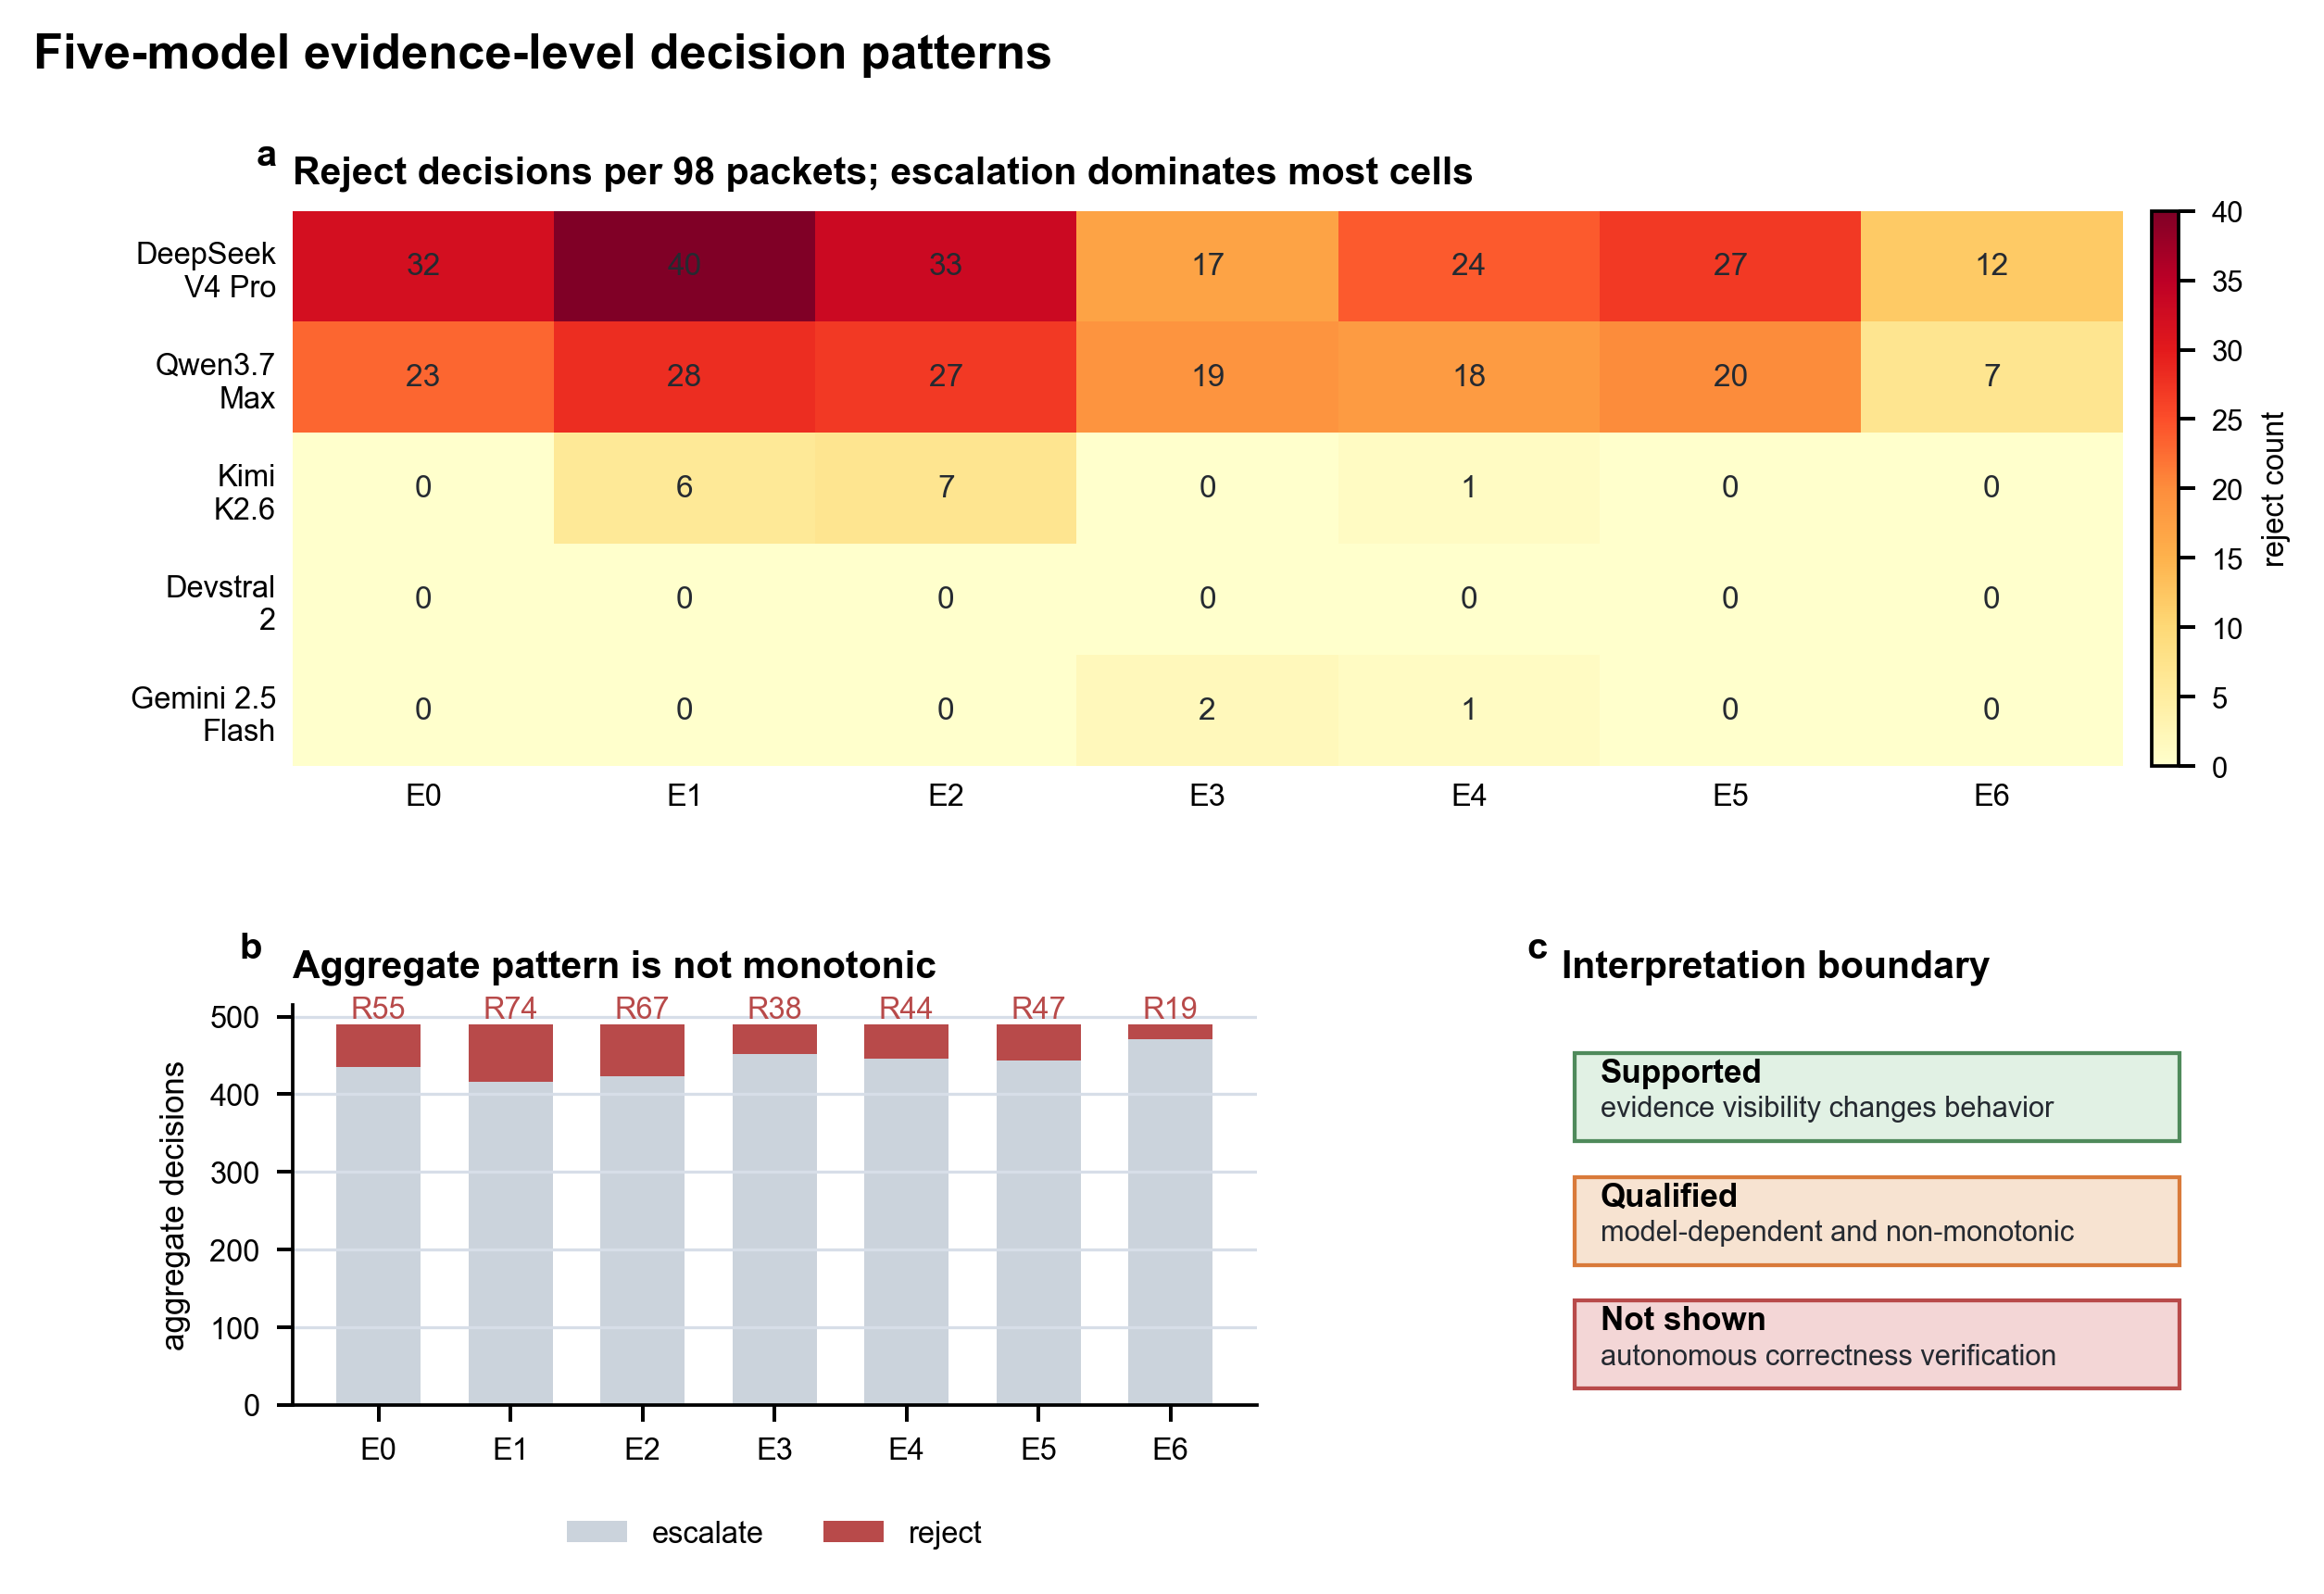
\includegraphics[width=\columnwidth]{../figures/ccfc/ccfc_fig2_decision_patterns.png}
\caption{Accept-aware and no-verdict metric evidence.}
\label{fig:apsec-2}
\end{figure}

The three-model result supports an evidence-visibility claim, not a monotonic correctness claim. More evidence changed policy behavior and unlocked acceptance, but DeepSeek's E4-E5 conservatism and the shared partial/regression false accepts show that visible evidence did not become a correctness oracle.

\subsection{Verdict-like evidence affected policy behavior}

The E6 ablation is a separate verdict-field ablation package rather than the repaired v0.3 E0-E6 main table. It compares the deterministic rule-only visible-tool baseline, full E6 model conditions, and E6-no-verdict conditions to test whether model decisions add value beyond following visible tool verdict fields. Therefore, the DeepSeek E6-full row below should be read as ablation evidence, while the repaired v0.3 DeepSeek E6 row in Section 5.1 is the main E0-E6 evidence-visibility result.

\begin{table*}[t]
\centering
\scriptsize
\setlength{\tabcolsep}{2pt}
\caption{E6 deterministic and no-verdict ablation.}
\label{tab:apsec-4}
\begin{tabularx}{\textwidth}{YYYYYYYY}
\toprule
condition & accept & reject & escalate & accepted precision & correct recall & false accept rate & escalation rate \\
\midrule
Rule-only visible-tool & 25 & 73 & 0 & 80.00\% & 95.24\% & 6.49\% & 0.00\% \\
DeepSeek E6-full & 23 & 75 & 0 & 82.61\% & 90.48\% & 5.19\% & 0.00\% \\
DeepSeek E6-no-verdict & 11 & 73 & 14 & 100.00\% & 52.38\% & 0.00\% & 14.29\% \\
Qwen E6-full & 24 & 74 & 0 & 83.33\% & 95.24\% & 5.19\% & 0.00\% \\
Qwen E6-no-verdict & 23 & 74 & 1 & 82.61\% & 90.48\% & 5.19\% & 1.02\% \\
\bottomrule
\end{tabularx}
\end{table*}

Qwen E6-full and rule-only produced similar correct recall, accepted precision, and false accept rates. Qwen E6-no-verdict remained close to Qwen E6-full. DeepSeek E6-no-verdict removed false accepts in this cohort, but correct recall dropped to 52.38\% and escalation increased to 14.29\%. The safer behavior therefore appears to be partly abstention-driven rather than strict semantic discrimination.

This is an important negative result for the LLM-verifier claim. The deterministic rule-only baseline was already strong: it reached 95.24\% correct recall and 80.00\% accepted precision, compared with 95.24\% and 83.33\% for Qwen E6-full. The goal of EVP-8 is not to show that LLMs dominate rule-only tool summaries, but to expose when LLM decisions collapse into tool-following, abstention, or prompt-induced conservatism. The current evidence therefore does not justify claiming a large LLM gain over the tool summary. The value of the LLM conditions in this draft is narrower: they expose how model policy changes when verdict-like fields are removed or challenged, and they show whether risky accepts are routed to escalation rather than autonomous acceptance.

The Wilson intervals are wide, so the ablation should be read as bounded risk-policy evidence rather than as a ranking of model quality. The full CI table remains part of the analysis package rather than a main-body table.

\subsection{Tool-contestation shifted risky accepts to escalation, not strict correction}

On the EVP-8-HARD cohort, tool-contestation evaluated 47 candidates for both Qwen and DeepSeek. For the known tool false-accept opportunity set, DeepSeek shifted 9 tool false accepts to 9 escalations and 0 strict rejects. Qwen shifted 9 tool false accepts to 8 escalations, with 0 strict rejects and 1 repeated accept.

This result supports safe handling through escalation. It does not support a claim that tool-contestation reliably identifies semantic incorrectness, because strict correction remained zero for both models.

The opportunity-set Wilson intervals are wide and are retained in the analysis package rather than expanded into a separate main-body table.

\subsection{Coverage-contestation removed repeated false accepts by becoming highly conservative}

The current-98 coverage-contestation condition tested whether a stronger prompt could challenge visible-test-only acceptance without changing the frozen E6/no-verdict packet set. It removed repeated false accepts for Qwen, DeepSeek, and Gemini, reducing the false accept rate on 77 non-correct candidates to 0.00\% for all three models. This is prompt-sensitivity evidence, not a new main result, because the same condition also collapsed correct-patch acceptance. DeepSeek and Gemini accepted no correct patches, and Qwen accepted only 2 of 21 correct patches.

The result answers a narrow prompt-setting question. A model can be instructed to challenge coverage sufficiency and avoid visible-test-only acceptance on this frozen cohort, but the observed mechanism is mostly conservative triage rather than semantic discrimination. Therefore the paper should not claim that coverage-contestation improves autonomous verification. The supported claim is that prompt framing can move false-accept risk into reject/escalate outcomes while imposing a large correct-recall cost.

\subsection{A hard-negative stress matrix reduced false accepts through escalation}

After the current-98 prompt-sensitivity result, we constructed a separated hard-negative stress cohort to test visible-pass/hidden-fail cases more directly. The cohort contains 31 hidden-failing candidates across PySnooper, cookiecutter, and scrapy. The visible-tool baseline accepted all 31 cases. Because the scrapy cases are curated no-API stress-source partial variants, this is a hard-negative stress-test supplement rather than a pure agent-generated realistic cohort.

Across Qwen, DeepSeek, and Gemini, the current merge-gate prompt produced 62 repeated false accepts in 93 model-condition records. The coverage-contestation prompt reduced repeated false accepts to 12/93. The reduction came entirely through escalation: strict rejects remained 0 in both conditions.

\begin{table*}[t]
\centering
\scriptsize
\setlength{\tabcolsep}{2pt}
\caption{Hard-negative stress matrix aggregate results.}
\label{tab:apsec-5}
\begin{tabularx}{\textwidth}{YYYYYY}
\toprule
condition & records & repeated false accepts & strict rejects & safe escalations & safe handling \\
\midrule
Current prompt & 93 & 62 (66.67\%) & 0 (0.00\%) & 31 (33.33\%) & 31 (33.33\%) \\
Coverage prompt & 93 & 12 (12.90\%) & 0 (0.00\%) & 81 (87.10\%) & 81 (87.10\%) \\
\bottomrule
\end{tabularx}
\end{table*}

This stress result strengthens the risk-triage interpretation. It shows that the stronger prompt can route many visible-pass/hidden-fail candidates away from autonomous acceptance, including all Gemini stress cases and all DeepSeek stress cases. It does not show semantic correction, because no condition strictly rejected the hard negatives. Correct recall is also undefined in this all-negative cohort.

\subsection{E6 false accepts were concentrated in partial and regression negatives}

The most important failure mode is not the average E6 score but the remaining E6 false accepts among 77 non-correct candidates. Aggregate false-accept anatomy shows that Qwen and DeepSeek each accepted three partial fixes and one regression patch, while Gemini accepted four partial fixes and one regression patch. In the single regression negative included in EVP-8, all three repaired models accepted it at E6; this is a severe failure signal, not a statistical claim about regression-safety failures. The partial-fix rows show a broader semantic-incompleteness pattern concentrated in youtube-dl tasks.

\begin{table*}[t]
\centering
\scriptsize
\setlength{\tabcolsep}{2pt}
\caption{False-accept anatomy and representative case groups.}
\label{tab:apsec-6}
\begin{tabularx}{\textwidth}{YYYY}
\toprule
project/task & negative type & models accepting & likely cause \\
\midrule
thefuck / thefuck\_1 & Regression patch & DeepSeek, Gemini, Qwen & visible E6 evidence missed a hidden P2P-broad regression \\
youtube-dl / youtube-dl\_11 & Partial fix & DeepSeek, Gemini & visible tests encouraged acceptance despite partial semantic repair \\
youtube-dl / youtube-dl\_16 & Partial fix & DeepSeek, Gemini, Qwen & visible tests encouraged acceptance despite partial semantic repair \\
youtube-dl / youtube-dl\_20 & Partial fix & DeepSeek, Gemini, Qwen & visible tests encouraged acceptance despite partial semantic repair \\
youtube-dl / youtube-dl\_6 & Partial fix & Gemini, Qwen & merge-gate summary did not expose the remaining semantic gap \\
\bottomrule
\end{tabularx}
\end{table*}

The sanitized case-level export records candidate id, project, task, negative type, E6 decision, no-verdict decision where available, and compressed rationale categories, but excludes raw response text, full rationale text, rendered prompts, patch diffs, and credentials. The table supports failure anatomy, not a claim that the complete model rationale has been audited semantically.

\section{Discussion}

The main implication is that LLM patch verification should be evaluated with explicit evidence boundaries. The same candidate patch may be treated differently when visible tests, regression checks, diagnostics, or deterministic tool summaries are introduced. Reporting only an aggregate accept/reject rate would hide this dependence.

The results also clarify the role of escalation. Escalation can be useful for software-quality workflows because it routes risky cases away from autonomous acceptance. However, escalation is not strict correction, and aggressive contestation can destroy correct-patch recall. This distinction matters for deployment: a verifier that escalates risky candidates may reduce unsafe automation, but it has not proven semantic incorrectness or preserved useful acceptance.

The strongest current contribution is methodological. EVP-8 provides a reproducible way to separate model-visible evidence from hidden evaluator labels, report accept/reject/escalate outcomes, and connect each claim to a validity gate. This is why the paper is framed as a controlled protocol and measurement study rather than as a new repair or verification algorithm.

Several reviewer concerns remain bounded rather than eliminated. The cohort is small, Wilson intervals are wide, repaired Qwen, DeepSeek, and Gemini are the main model conditions, majority-vote cannot be computed from the current tracked summaries, and the hard-negative stress matrix is a stress-test supplement rather than a pure realistic agent-patch cohort. Most importantly, the current paper-facing main result is three-model but still not broad-model. These are not hidden weaknesses; they are the boundary conditions under which the current claims are valid.

\begin{figure}[t]
\centering
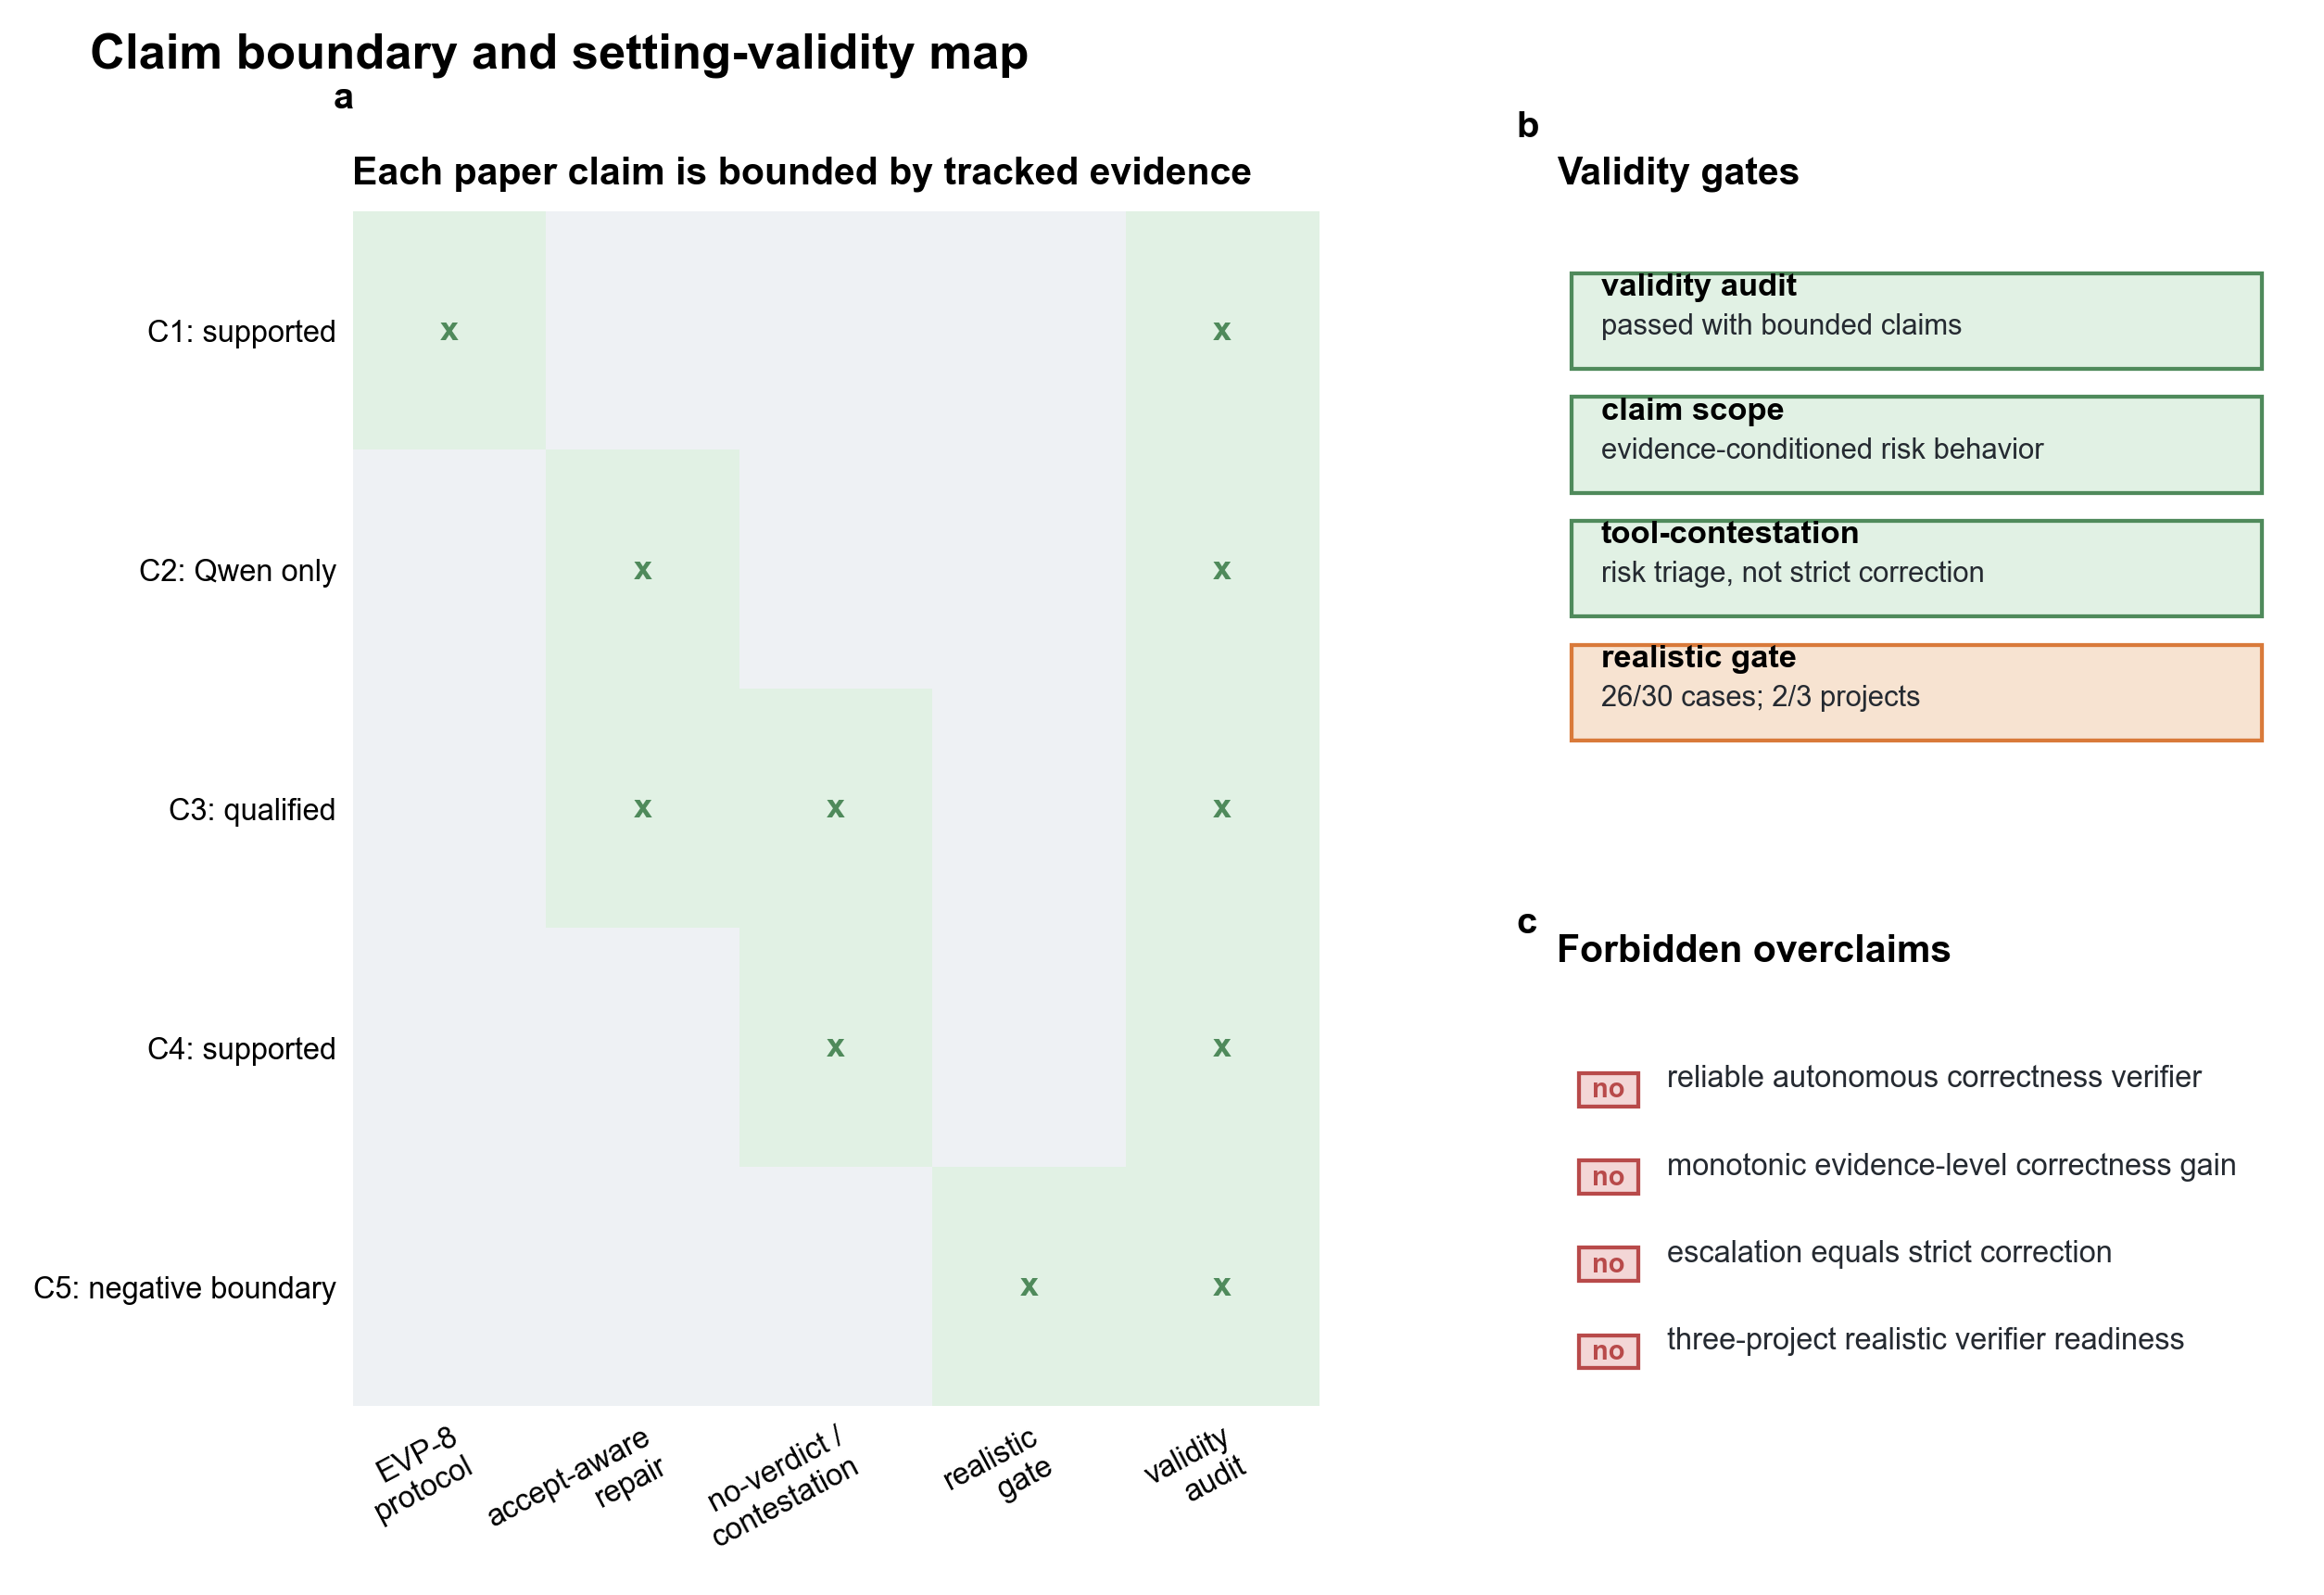
\includegraphics[width=\columnwidth]{../figures/ccfc/ccfc_fig3_claim_boundary.png}
\caption{Claim boundary and setting-validity map.}
\label{fig:apsec-3}
\end{figure}

\section{Threats to Validity}

\textbf{Internal validity.} Prompt wording, output schema, and evidence formatting may influence decisions. The study mitigates this risk through frozen packets, tracked prompt-boundary checks, parse-validity audits, raw-output-free summaries, and post-decision label joins. These controls reduce setup risk but do not make the results independent of the evaluated protocol versions.

\textbf{Construct validity.} The accept/reject/escalate decision space simplifies real review workflows. Escalation is a routing outcome, not proof of semantic rejection. Hidden evaluator labels are used only for post-decision analysis and should not be interpreted as model-visible truth.

\textbf{External validity.} The main evidence comes from a 98-candidate EVP-8 cohort, an EVP-8-HARD controlled cohort, a 31-case hard-negative stress matrix, and selected model conditions. The repaired E0-E6 main result now covers Qwen, DeepSeek, and Gemini, but it is still not a broad-model result. The hard-negative stress matrix reaches three projects, but the scrapy cases are curated no-API stress-source variants, so it should not be generalized as a pure agent-generated realistic cohort. The results therefore support bounded evidence-conditioned risk behavior in a controlled patch-verifier study, not universal LLM patch-verifier reliability.

\textbf{Baseline validity.} Rule-only visible-tool is the completed deterministic baseline. Always-* and uniform-random policies are reference policies. Majority-vote and a separate deterministic E0/no-tool verifier remain unavailable under the current tracked-summary boundary.

\section{Conclusion}

This paper introduces EVP-8 as a hidden-evaluator evidence-visibility protocol for candidate patch verification. The repaired Qwen, DeepSeek, and Gemini v0.3 results show that visible executable and tool evidence can unlock correct-patch acceptance while retaining false-accept risk and model-dependent caution. E6 ablations, tool-contestation, coverage-contestation, and the hard-negative stress matrix further show that verdict-like evidence and prompt framing can shape policy behavior, and that safer handling often occurs through escalation rather than strict semantic correction. The contribution is a reproducible software-engineering protocol for measuring evidence-conditioned risk behavior in a controlled LLM patch-verifier study, not a claim of autonomous patch correctness verification.


\bibliographystyle{IEEEtran}
\bibliography{apsec_references}
\end{document}
